\documentclass[11pt, oneside]{article}   	% use "amsart" instead of "article" for AMSLaTeX format
%\usepackage{geometry} 
\usepackage[margin=0.8in]{geometry}                		% See geometry.pdf to learn the layout options. There are lots.
\geometry{letterpaper}                   		% ... or a4paper or a5paper or ... 
%\geometry{landscape}                		% Activate for rotated page geometry
\usepackage[parfill]{parskip}    		% Activate to begin paragraphs with an empty line rather than an indent
\usepackage{graphicx}				% Use pdf, png, jpg, or eps§ with pdflatex; use eps in DVI mode
								% TeX will automatically convert eps --> pdf in pdflatex		
\usepackage{amssymb}
\usepackage{amsmath}
\usepackage{hyperref}

%SetFonts

%SetFonts
%\vspace{-5ex}

%\title{\vspace{-10ex} Research Proposal: Computational Morality \vspace{-5ex}}
\title{Competition: Hindi to English Machine Translation System}

\author{
    Shruti Sharma  \\ 
    20111061\\
   {\tt \{shruti20\}@iitk.ac.in}\\
{Indian Institute of Technology Kanpur (IIT Kanpur)}
}


\date{\today}							% Activate to display a given date or no date

\begin{document}
\maketitle

\abstract{Neural Machine Translation is the task of converting text from source language to target language. This assignment aims to evaluate different Hindi-to-English NMT approaches using sequence-to-sequence models and transformers. Seq2Seq models have 2 RNNs working together, that might use attention mechanism for performance improvement. BLEU score and METEOR score are used as accuracy metrics. Best rank was 11 with METEOR score 0.219 in Phase 2 using 2 layer stacked Bidirectional LSTM. This score is exactly equal to the SOTA score of Hi-En NMT mentioned in the provided document. }

\section{Competition Result}
\textbf{Codalab Username:} S\_20111061 \\
\textbf{Final leaderboard rank on the test set:} 13 \\
\textbf{METEOR Score wrt to the best rank:} 0.301 \\
\textbf{BLEU Score wrt to the best rank:}  0.0839\\ 
\textbf{Link to the CoLab/Kaggle notebook:}
\url{https://colab.research.google.com/drive/1RR4Zs4dyDnRHABwdwLml0qZ7sU6-WMGD?usp=sharing}

\section{Problem Description}
Language barrier is one of the challenge world faces for communication. Language Translation helps solve this issue and so has global effect. To overcome this barrier, there's a need of efficient and reliable translation model. Translation is modelled as $argmax_{y}{P(y|x)}$. There exists techniques based on lexical, syntactic and semantic rules (Rule Based Machine Translation) and techniques using statistical models for translation (Statistical Machine Translation). Although, this assignment aims to create a Neural Machine Translation model for Hindi to English translation as NMT requires less data than other methods and still exhibit satisfactory results. All the implementation is done in Python3's machine learning package PyTorch. Codes are run on GPU because of resource-hungry models and batchification of training process.

\section{Data Analysis}
The parallel corpus for training has been taken from publicly available sources \url{https://opus.nlpl.eu/} and \url{http://www.opensubtitles.org/ }\\
It has 101322 lines with English vocabulary size of 50854 and Hindi vocabulary size of 33968. Data is in Hindi-English sentence pair format as,
\begin{center}
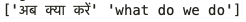
\includegraphics[scale=0.58]{eg.png} 
\end{center}
\newpage
Plot to visually confirm Zipf's Law
\begin{center}
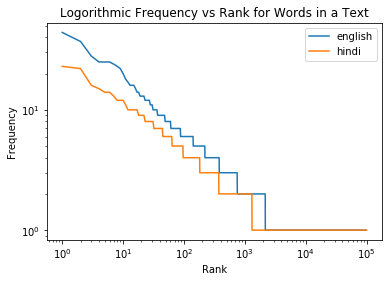
\includegraphics[scale=0.6]{zipf.png}
\end{center}
Most frequent words in English corpus and their counts
\begin{center}
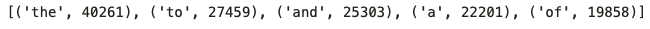
\includegraphics[scale=0.6]{eng.png} 
\end{center}
Most frequent words in Hindi corpus and their counts
\begin{center}
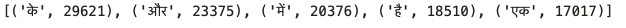
\includegraphics[scale=0.6]{hinfreq.png} 
\end{center}
Plot of number of “meanings” of a word in Wordnet vs its use in our English corpus
\begin{center}
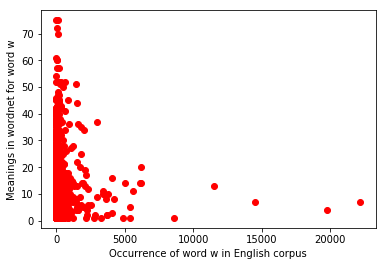
\includegraphics[scale=0.6]{meaning.png}
\end{center}

\section{Model Description}
\subsection{Sequence-to-Sequence Models\cite{sutskever2014sequence}}

Sequence-to-Sequence (Encoder-Decoder) models are the simplest ones to be used for NMT. They work on the principle of reading symbols from input sequence one at a time using a Recurrent Neural Network (RNN) and predict words for target sequence using another RNN. It models language translation conditionally as,
\begin{align*}
P(y|x) = P(y_1|x) P(y_2 | y_1,x) .... P(y_n | y_1, ..., y_{n-1}, x)
\end{align*}
where x is source sentence and y is target.
RNN cells use the memory (hidden state) and their own outputs as inputs for next step. They can be unrolled to store the sentences as sequence in both source and target languages, without having us to worry about the sequence length and so are apt for use in translation tasks. Using a single RNN will not aid in this case. They can map sequences to sequences if alignment is known beforehand. Encoder processes the input sequence and compresses it entirely into a context (thought) vector of fixed length (final hidden vector). This context vector is used to initialize the decoder's initial hidden state to make predictions. It predicts one word at a time using above conditional probability where new word is predicted using previously predicted words and source sentence vectors. A Softmax function is applied on the predictions over all the words in vocabulary.  \\
The tokenized input sequence is passed through the encoder-decoder architecture. Experiments were performed using bidirectional GRU and LSTM as RNN layers. In variant, 2 RNN cells with one dropout layer between them also have been tried.

\subsubsection{Long Short Term Memory}
Encoder bidirectional LSTM reads the input sequence and summarizes information in internal state vectors - hidden state and cell state. The cell state makes LSTM more useful. The gates connected to it control flow of information as needed. The input to encoder are all tokens in source vocabulary. The encoder outputs are discarded and final state vectors are used to initialize the decoder, which is also a LSTM. A variant of LSTM by stacking another layer of LSTM encoder and decoder was also used. Bidirectional LSTM works on the principle that output at a moment can depend on past as well as future data. So in vanilla LSTM, two hidden layers of opposite directions are connected to same output.

\subsubsection{Gated Recurrent Unit}
Encoder GRU has only one internal state - hidden state. Intermediate encoder outputs are rejected and final state vector is used to initialize the decoder which is effective for short sequences but gets difficult in summarizing long sequences in a single vector.

\subsubsection{Attention Mechanism}
It is easy for humans to relate different parts of input sentence and transform it accordingly into a valid output. For neural models, this is done using attention mechanism. It ``learns" these mappings through gradient descent and backpropagation.\\
Fixed-length context/thought vectors of vanilla seq2seq models are unable to remember and correlate long sequences. Attention layer acts as an interface between encoder and decoder, and use every intermediate encoder state to construct context vectors that are passed to decoder. The model can then selectively focus on important parts of input and learn the alignment between them. Bahdanau's\cite{bahdanau2016neural} alignment model introduces a matrix of weights that connects each input location to each output location. Attention calculation requires decoder's output from previous time step. Luong \cite{luong-etal-2015-effective} uses a global approach for attention that attends all source words and use each time step encoder's and decoder's output for attention calculation. It gives higher weights to those encoder hidden states that are more similar to current decoder hidden state.\\
A simple global attention has been used wherein decoder looks back at all hidden states of encoder to create memory vector. It uses this vector and it's own hidden vector to predict outputs. To use every encoder hidden state, a Softmax function is used to take weighted average of all indices in $L_x X 1$ alignment vector $a_t$ to create a probability vector $a'_t$. $L_x$ is the number of encoder hidden states being weighted over. Therefore,
\begin{align*}
a'_t = softmax(a_t)
\end{align*}
The context vector $d_t$ is weighted average over all encoder hidden states and is computed at each time step in decoder.
\begin{align*}
d_t = \sum_{s=0}^{L_x}  a'_t[s] * h_{t'=s}^E
\end{align*}
$d_t$ is then used with current decoder hidden state $h_t^D$ as,
\begin{align*}
\tilde{h}_t^D = tanh(W_{\tilde{h}} [d_t : h_t^D])
\end{align*}
The prediction vector $\hat{y}_t$ is,
\begin{align*}
\hat{y}_t = softmax(U\tilde{h}_t^D )
\end{align*}
$\tilde{h}_t^D$ is fed as the next step hidden state to RNN.


\subsection{Transformers}
Seq2Seq models (including LSTM) have problem dealing with long-range dependencies.The Transformer model \cite{vaswani2017attention}  mainly focus on self-attention mechanism to solve this, which models relationships between words in a sentence, irrespective of their position. They differ from Seq2Seq in not using any RNN but linear layers and handling input sequence at once, and not word by word.\\
Encoder and Decoder are replicated 6 times. Each encoder has 2 parts : Multi-head self-attention \& position-wise fully connected feed forward networks. It receives vectors of embedding dimension = 512. Both encoder-decoder add positional encoding to their embedded vectors and a residual connection followed by batch normalization. Residual connections add input of a layer element-wise with the output before passing it to next layer. This improves the gradient flow in backward pass. Positional encoding using sine and cosine transformations is needed to encode the ordering information of sequence. Residual connections make optimization easier. For residual connections, all sub-layers in the model, as well as the embedding layers, produce outputs of dimension 512.
 In each iteration, the decoder receives the encoder’s input and the decoder’s last output and uses both for the next step. Each encoder and decoder have fully-connected layers with RELU activation to make the layers learn new dependencies by itself.\\
Multi-headed attention used dot-product operation parallely across 8 projections. Self-attention is needed in encoder to focus on words that affect the next word the most. It is required in decoder to pay attention to previous word being generated, to correctly predict next words. Create query, key and value vectors for each word by multiplying embedding vectors with 3 matrices obtained during training. These matrices are initialised using Xavier initialisation. Query vector is represented as word vector of sentence and represents hidden state of decoder. Key vector represented as all words in sequence and represents hidden state of encoder. Value vector represents all words of sequence and defines attention weights of encoder hidden states. Q,K,V have dimension 64. Each column gives the probability score for each word wrt the scoring word. For attention between encoder and decoder, query is from previous decoder embedding layer and key and value are from encoder output.

\section{Experiments}

\subsection{Data Preprocessing}
Raw data has to be preprocessed to remove noise like non-ascii characters and punctuations and encode each line to ASCII and then decode to UTF-8. Some of the Hindi sentences had English alphabets in them. The cleaned data has 100926 lines. Since the sentence lengths can be quite large in corpus that can have adverse effect on sequence model, we constrain them by MAX\_LENGTH = 60.\\
NLTK tokenizer and IndicNLP library are used to clean, normalize and tokenize the data. For English, replace everything with space except (a-z, A-Z, “.”, “?”, “!”, “,”, ``-"). Extra spaces are removed. Abbreviations are expanded by mapping them through a dictionary.\\
The data is vectorized because this scales down the computation costs by several magnitudes. Using matrix operations for dealing with data will also prove beneficial in terms of performance gains.\\
``SOS" is used as start of sentence marker for target sequence and 	``EOS" is end of sentence marker. A class is used to map a word to its index and vice-versa. A unique vocabulary for each language is constructed. Words not present in training dataset are replaced by 	``UNK". For the batch length to be same, sentences are padded using ``EOS". Therefore, input sequences are represented as 2D-tensor of dimension $(batch size * max length)$.

\subsection{Training Procedure}
After dataset is preprocessed, it is split as 90\% for training and 10\% for validation. The sentences are then fed to encoder to prepare vectors. Minibatch Gradient Descent, an optimization algorithm, is used for training. To tackle the vanishing gradient problem that is common in RNNs, LSTMs are used. In case of GRU, RELU activation is used.\\
Teacher forcing (= 0.5) the actual target sequence to decoder, disregarding its predictions at that time step helps speed up the training process.\\
Optimizers tried : RMSProp, Adam, SGD\\
To predict accuracy of predicted translation to actual translation, CrossEntropy loss algorithm is used,
\begin{align*}
- \sum_{w=1}^S \sum_{e=1}^V y_{w,e} \log(\hat{y}_{w,e})
\end{align*}
where, $\hat{y}_{w,e}$ is predicted probability of vocab entry e on word w. $y_{w,e} = 1$ when vocab entry is correct word. $y_{w,e} = 0$ when vocab entry is not correct word. \\ 
For Bidirectional LSTM with 2 layers and attention decoder,
\begin{center}
\begin{tabular}{ ||c|c|| } 
 \hline
 Hyperparamter & Value \\ [0.5ex] 
 \hline\hline
 Batch Size & 32 \\
 \hline 
 Epochs & 12  \\ 
 \hline
 Hidden size & 512\\ 
 \hline
 Learning rate & 0.001 \\
 \hline
 Optimizer & Adam\\
 \hline
 Dropout & 0.1\\
 \hline
  Activation Function & Tanh \\
 \hline
  Training Time & 3 hours\\
 \hline
\end{tabular}
\end{center}

For single layer BiLSTM, 
\begin{center}
\begin{tabular}{ ||c|c|| } 
 \hline
 Hyperparamter & Value \\ [0.5ex] 
 \hline\hline
 Batch Size & 32 \\
 \hline 
 Epochs & 6  \\ 
 \hline
 Hidden size & 1080\\ 
 \hline
 Dropout & 0.1\\
 \hline
  Training Time & 1 hr for 1 epoch\\
 \hline
\end{tabular}
\end{center}

\bigskip

For Bidirectional GRU with 2 layers and attention decoder,
\begin{center}
\begin{tabular}{ ||c|c|| } 
 \hline
 Hyperparamter & Value \\ [0.5ex] 
 \hline\hline
 Iterations & 30000\\
 \hline
 Hidden size & 512\\ 
 \hline
 Learning rate & 0.001 \\
 \hline
 Optimizer & Adam\\
 \hline
 Dropout & 0.1\\
 \hline
 Activation Function & RELU \\
 \hline
  Training Time & 4 hours\\
 \hline
\end{tabular}
\end{center}

The latent dimensionality of encoding space was put to be 256, 512, 1024 and 1080. Although, 512 gave the best result.GRU was less expensive and fast than LSTM due to presence of single internal 
state.\\

\medskip
For transformers,
\begin{center}
\begin{tabular}{ ||c|c|| } 
 \hline
 Hyperparamter & Value \\ [0.5ex] 
 \hline\hline
 Batch Size & 64 \\
 \hline 
 Epochs & 12  \\ 
 \hline
 Embedding size & 512\\ 
 \hline
 Learning rate & 0.003 \\
 \hline
 Optimizer & Adam\\
 \hline
 Dropout & 0.1\\
 \hline
  Activation Function & RELU \\
 \hline
 Training Time & 3 hours\\
 \hline
\end{tabular}
\end{center}

\medskip
Greedy approach is used for predictions.

\section{Results}

The best performing model on test-set is 3-layered bidirectional LSTM with hidden size 512. As the depth of neural networks increases, the problem of vanishing and exploding gradients is being handled by residual connections in LSTM. The output of one LSTM is added to input and is forwarded as input to next LSTM. Attention models perform well but take longer time for training and hence are expensive. Adam optimizer gave better BLEU score than others as it not only controls the learning rate and momentum but also influences the rates such that performance is affected by the recent context.

On dev-set,
\begin{center}
\begin{tabular}{ ||c|c|c|c|| } 
 \hline
 Model & METEOR Score & BLEU score & Rank \\ [0.5ex] 
 \hline\hline
 BiLSTM (HS-512)& 0.179 & 0.005 & 16 \\
 \hline
 BiGRU & 0.067 & 0.000 & NA on Codalab \\
 \hline
 2 layer stacked BiLSTM (HS-512) & 0.222 & 0.0402 & 14 \\
 \hline
 Transformer &0.137 &0.037 &12\\
 \hline
\end{tabular}
\end{center}

On test-set,
\begin{center}
\begin{tabular}{ ||c|c|c|c|| } 
 \hline
 Model & BLEU Score & METEOR Score & Rank \\ [0.5ex] 
 \hline\hline
 Single layer  BiLSTM (HS-1080) & 0.0184 & 0.169 & 34\\
 \hline
 2 layer stacked BiLSTM (HS-1024) & 0.0598 & 0.274 & 23 \\
 \hline
  2 layer stacked BiLSTM (HS-512) & 0.0796 & 0.306 & 17 \\
  \hline
 3 layer stacked BiLSTM (HS-512) & 0.0839 & 0.301 & 13\\
 \hline
\end{tabular}
\end{center}

\section{Error Analysis}
Improvement in BLEU score\cite{bleu} doesn't ensure better translations \cite{Zhang04interpretingbleu/nist}. For the statement,\begin{center}

\includegraphics[scale=0.5]{hin.png} 
\end{center}
BiLSTM with hidden dimension 512 gave the prediction ``this crazy deep sense of madness
" but with hidden dimension 1024 gave ``this madness is crazy" although the former model had better BLEU score. This kind of evaluation can be extended to multiple human eyes to test the accuracy of the models. Model's superiority can also be checked by randomly translating sentences during training and comparing with original translation. Increasing the layers improves efficiency of the system. That is why a 3 layer stacked bidirectional LSTM gives best performance. It is able to capture and correlate information in a better way than rest of the models.
\\
BLEU and METEOR scores speak about the quality of translation. In research, it has been shown that BLEU favours SMT systems more than RBMT and NMT although they produce more fluent translations than SMT. BLEU score is based on matching text strings. That is, larger cluster of words to match gives higher BLEU score but BLEU is less linguistically informed and compares human translation with machine translation. It doesn't count subwords of same source as correct alternative. METEOR solves this issue by including some additional step by considering synonyms, word order changes and using stems of words for comparison.
\\
The results were not consistent due to lack of computing resources as training had to be done in breaks. The performances could have been better if given more time to train and with better quality dataset. Hyperparameter tuning and training takes a lot of time and analysis of results becomes difficult. \\
The other difficulty is in learning rare words. In the current system, the unknown words are replaced by ``UNK" but sparse inputs need to be handled better. 
\\
The model's cross-entropy loss was monitored to test their performance. Below are the plots for the same.
\subsection{Plots}
\subsubsection{Loss}
For 2 layer stacked BiLSTM, we can see that training loss decreases consistently but validation loss remains almost constant.
\begin{center}
\includegraphics[scale=0.6]{Loss512LSTM.png}
\end{center}

\subsubsection{Accuracy}
For long sentences, predictions aren't that well using Seq2Seq.
\begin{center}
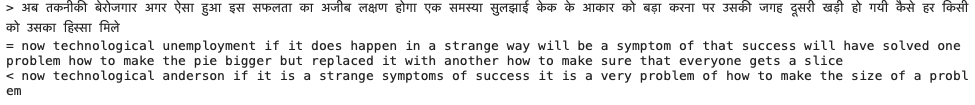
\includegraphics[scale=0.6]{long}
\end{center}
but quite excellent for small word predictions. Here, although the provided pair was not correct translation, but BiLSTM predicted it perfectly.  [$>$ : original sentence, = : original target,$ <$ : predicted sentence]
\begin{center}
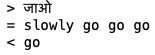
\includegraphics[scale=0.6]{small}
\end{center}

\section{Conclusion} 
With increase in computational capabilities, NMT has proved significant for translation models. The encoder-decoder architecture has given incredible accuracy. With addition of attention architecture, it is further improved. This assignment aims to enhance the NMT model. By increasing a larger training dataset, batchifying the training procedure, monitoring the validation set accuracy during training, and tweaking the model hyperparameters, an ultimate NMT model can be created.\\
To improve the performance of model in terms of BLEU score, Adam optimizer should be used on larger corpus. Attention models give better results in fewer epochs than models without attention. The Transformer model which uses only attention layers and discards convolutional and recurrent layers, are highly parallelizable and efficient.\\

\textbf{Future Directions}
\begin{enumerate}
\item Exploring other optimal neural architectures for translation models like ConvS2S and attention mechanism like local attention.
\item Using reversed input sequence for training the model \cite{luong-etal-2015-effective}.
\item Using pre-trained word embeddings to allow words with similar meaning have same distributed representation.
\item Using advanced algorithms to decide the learning rate.
\item Using beam search like conditional generation of output sequence using input sequence and output generated so far.
\item Use larger training set.
\end{enumerate}
\bibliography{references} 
\bibliographystyle{ieeetr}

\end{document}  